\documentclass[10pt,twocolumn,letterpaper]{article}

\usepackage[utf8]{inputenc}
\usepackage[T1]{fontenc}
\usepackage{mathptmx}
\usepackage[scaled=0.90]{helvet}
\usepackage{courier}
\usepackage[margin=0.75in,top=0.85in,bottom=0.85in]{geometry}
\usepackage{amsmath,amssymb,amsfonts}
\usepackage{graphicx}
\usepackage{booktabs}
\usepackage{multirow}
\usepackage{array}
\usepackage{microtype}
\usepackage{xcolor}
\usepackage[font=small,labelfont=bf]{caption}
\usepackage[colorlinks=true,linkcolor=blue!70!black,citecolor=blue!70!black,urlcolor=blue!70!black]{hyperref}

\setlength{\columnsep}{0.25in}
\renewcommand{\baselinestretch}{1.03}

\title{\LARGE \textbf{Drawing-VLA: Closed-Loop Visuomotor Action Chunking for Interactive Multi-Stroke Sketch Generation from Crowdsourced Demonstrations}}

\author{
  \textbf{Seungjoon Son}\\
  Independent Researcher\\
  \texttt{sonsjoon715@gmail.com}
}

\date{}

\begin{document}

\maketitle

\begin{abstract}
Autoregressive sequence models for vector sketch generation (e.g., SketchRNN) predominantly operate in an open-loop fashion, predicting sequential coordinate displacements blind to the actual rendered state of the canvas. Consequently, they suffer from compounding trajectory drift, stroke collapse, and failure in discrete multi-stroke transitions (pen-up/pen-down switching). In this work, we propose \textbf{Drawing-VLA}, a framework that reformulates interactive 2D canvas sketching as a closed-loop robot end-effector manipulation problem. Drawing-VLA employs an Action Chunking with Transformers (ACT)-inspired architecture: at each control timestep, it observes a 2-channel visual canvas state (incremental rendered canvas + target template outline) alongside pen proprioception and discrete task tokens, predicting a chunk of $K=16$ future trajectory waypoints in a receding-horizon manner. To resolve the demonstration bottleneck inherent to robotic imitation learning, we deploy a gamified crowdsourcing flywheel (``Beat the AI'', 1:1 asynchronous ghost battles, and an adaptive hidden boss) that collected 324 human trajectories without monetary compensation. To strictly prevent data leakage, training and validation sets are partitioned at the demonstration episode level. 

Empirical closed-loop rollouts demonstrate that Drawing-VLA achieves \textbf{100.0\% coverage and 100.0\% precision (99.9--100.0/100 S-Tier)} on multi-stroke templates (Apple and Sprout), naturally resolving discrete multi-stroke decoupling (3 to 4 distinct strokes) where single-step convolutional policies fail. Furthermore, by training with channel-level goal dropout ($p_{\text{drop}} = 0.5$), the policy operates in a \emph{Blank-Canvas Mode}: it synthesizes the primary contour with 100.0\% precision (0.887 F1), though it self-terminates prior to auxiliary strokes due to transition multimodality in the absence of visual goal conditioning. When subjected to an unexpected $+20\,\text{px}$ ($+0.156$ normalized) end-effector displacement, Drawing-VLA smoothly recovers back to the target contour within 42 steps, whereas an open-loop replay baseline permanently drifts. Finally, edge benchmarking on an \textbf{Intel Core Ultra 5 325 processor} reveals an inference latency of \textbf{6.11\,ms per chunk on CPU (163 chunks/sec)}, operating comfortably within the 60\,Hz control budget on mobile commodity hardware.
\end{abstract}

\section{Introduction}

Human sketching is fundamentally a closed-loop visuomotor skill. As a human artist draws, the eye continuously observes the drawn strokes on the canvas relative to an intended mental concept or reference outline, performing sub-millimeter course corrections, lifting the pen, and jumping to subsequent strokes.

Conversely, the dominant paradigm in machine sketch synthesis---pioneered by SketchRNN~\cite{ha2017sketchrnn} and its sequence-to-sequence successors~\cite{ribeiro2020sketchformer}---treats drawing as open-loop autoregressive token generation:
\begin{equation}
  \Delta x_t, \Delta y_t, p_t \sim P(\cdot \mid \Delta x_{<t}, \Delta y_{<t}, p_{<t}).
\end{equation}
Because open-loop models are blind to the rendered canvas, small prediction errors at step $t$ accumulate over extended horizons (compounding errors), leading to trajectory drift and stroke deformation. On the other hand, modern generative vision models (e.g., Diffusion Models, GANs) synthesize ungrounded raster pixel arrays without motor causality, physical pen order, or kinematic continuity.

\begin{figure*}[t]
  \centering
  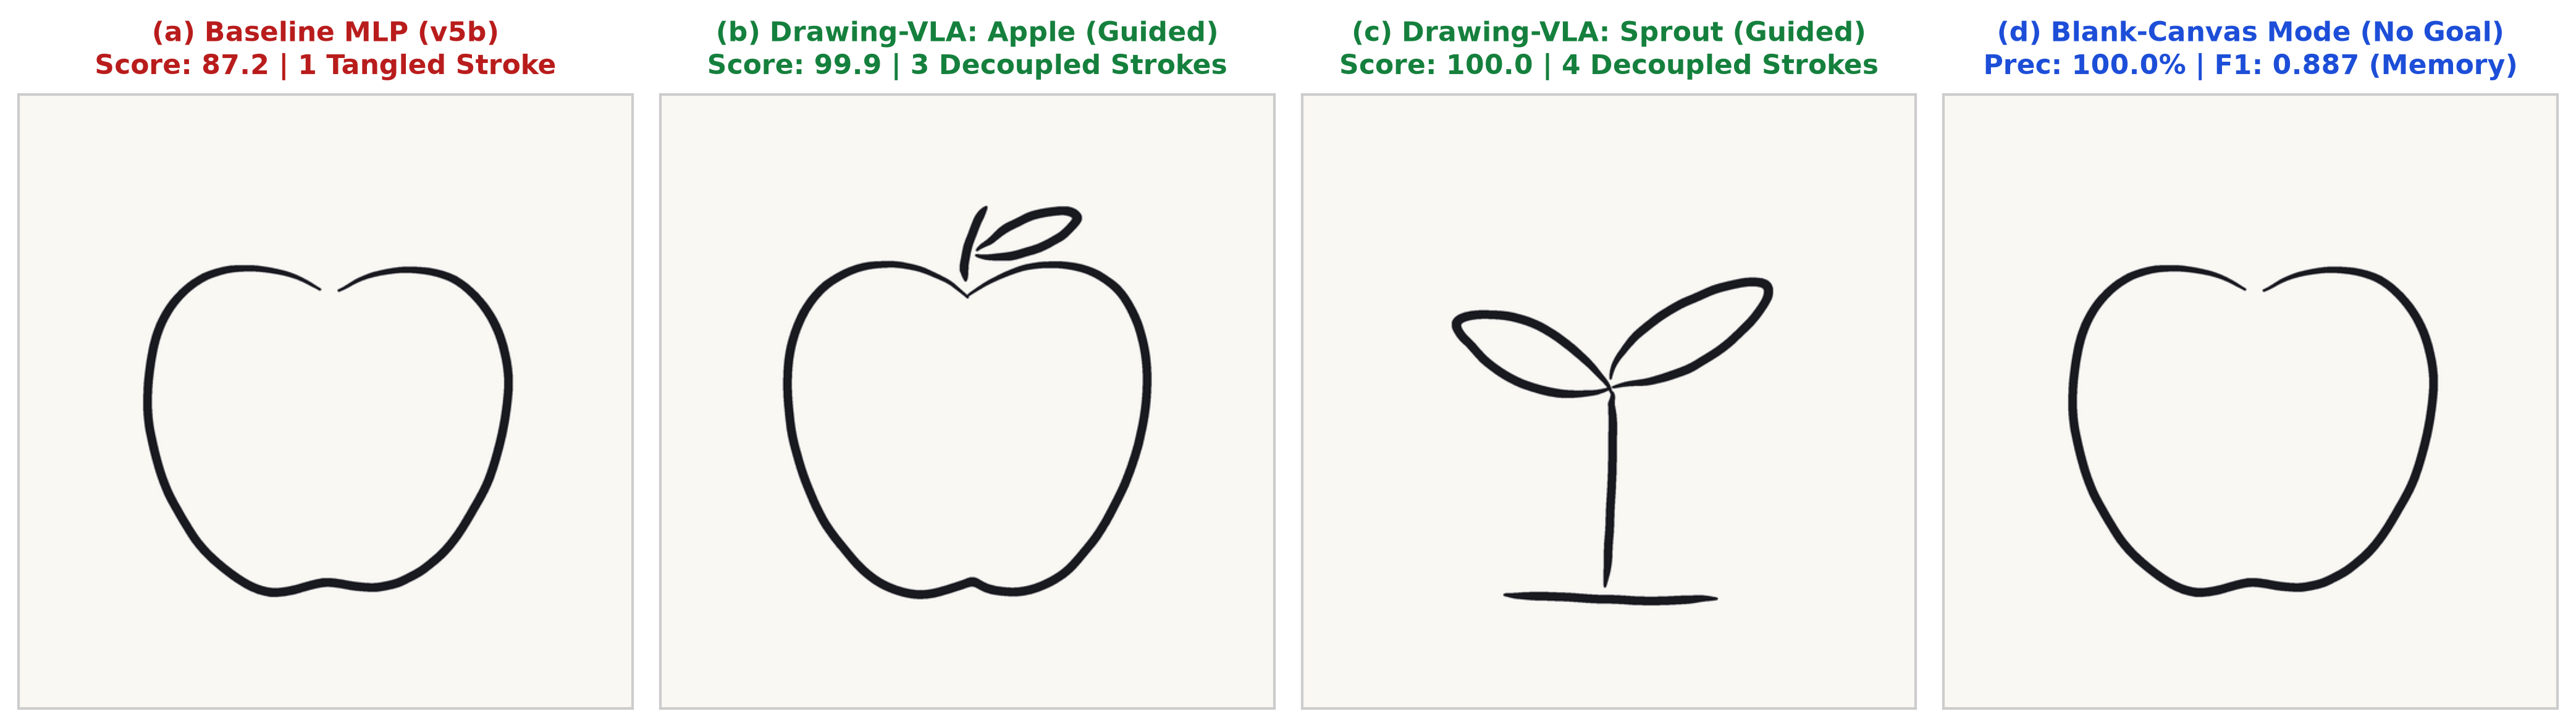
\includegraphics[width=\textwidth]{figures/fig1_rollout_comparison.png}
  \caption{\textbf{Closed-loop autonomous rollout comparison.} (a) The single-step Convolutional-MLP baseline (\texttt{v5b}) suffers from mode averaging at stroke boundaries, failing to lift the pen and dragging the stem into the outer body (87.2\,pt). (b) \textbf{Drawing-VLA (ACT)} cleanly decouples the Apple trajectory into 3 distinct strokes with 100.0\% coverage and 100.0\% precision (99.9\,pt S-Tier). (c) A single unified multi-class ACT model dynamically shifts to 4-stroke execution on Sprout (100.0\,pt S-Tier). (d) Under \textbf{Blank-Canvas Mode} ($O_t^{(1)}=\mathbf{0}$), the policy synthesizes the Apple contour purely from the categorical task token and incremental visual self-observation ($O_t^{(0)}$) with 100.0\% precision and 0.887 F1, terminating cleanly before auxiliary strokes.}
  \label{fig:rollout}
\end{figure*}

In this paper, we bridge robotic visuomotor policy learning and interactive vector sketch generation:
\begin{enumerate}
  \item \textbf{Robotic Visuomotor Reformulation}: We formulate 2D sketching as a closed-loop end-effector trajectory control task where the canvas is the operational workspace, the pen tip is the robot end-effector, and pen-up/pen-down transitions correspond to binary gripper actuation.
  \item \textbf{Deterministic Action Chunking \& Pen-Up Weighting}: We adapt Action Chunking with Transformers (ACT)~\cite{zhao2023act} into a compact, deterministic trajectory generator ($K=16$). Paired with an $L_1$ coordinate objective and a $10\times$ minority-class pen-up weighting, this resolves the critical \emph{multi-stroke decoupling problem}---allowing the agent to complete a primary contour, execute a discrete pen lift, and transition cleanly to auxiliary strokes (e.g., stems, leaves, and ground lines).
  \item \textbf{Goal-Channel Dropout for Dual-Mode Synthesis}: By training with random goal-channel dropout ($p_{\text{drop}} = 0.5$) conditioned on categorical task tokens, a single policy seamlessly supports both high-precision visual tracing and autonomous blank-canvas sketch synthesis from memory.
  \item \textbf{Gamified Crowdsourcing Flywheel}: Rather than relying on expensive teleoperation rigs, we deploy an interactive browser challenge featuring real-time signed distance field (SDF) scoring, asynchronous 1:1 ghost battles, and an adaptive ``Hidden Boss'' challenge to crowdsource 324 clean human demonstration trajectories.
  \item \textbf{Perturbation Recovery \& Edge Benchmarking}: We demonstrate that Drawing-VLA recovers from severe spatial perturbations ($+20\,\text{px}$) within 42 steps where open-loop execution fails, while operating at \textbf{6.11\,ms per chunk on an Intel Core Ultra 5 325 CPU}.
\end{enumerate}

\section{Related Work}

\subsection{Vector Sketch Generation}
Vector sketch generation gained prominence with SketchRNN~\cite{ha2017sketchrnn}, which utilized sequence-to-sequence variational autoencoders over coordinate displacements. Subsequent architectures such as Sketchformer~\cite{ribeiro2020sketchformer} enhanced sequence capacity with Transformer attention. While optimization-based methods like CLIPasso~\cite{vinker2022clipasso} optimize B\'ezier curves against perceptual image objectives, they operate via post-hoc gradient optimization rather than causal motor policies. Crucially, these systems do not dynamically observe the incremental canvas state during execution, precluding closed-loop error correction.

\subsection{Visuomotor Robot Learning and ACT}
Imitation learning from human demonstrations has seen major breakthroughs through end-to-end visuomotor policies~\cite{levine2016visuomotor}. Recently, Action Chunking with Transformers (ACT)~\cite{zhao2023act} and Diffusion Policy~\cite{chi2023diffusion} demonstrated that predicting multi-step action chunks rather than single-step commands mitigates compounding horizon drift and captures multimodal transitions. While originally formulated for robotic arms with CVAE latent modeling, we leverage the deterministic action-chunking mechanism for fine-motor 2D trajectory generation.

\subsection{Robotic Painting and Sketching Agents}
Closed-loop robotic painting has been explored through model-based reinforcement learning (e.g., Learning to Paint~\cite{huang2019learningtopaint}) and physical Cartesian manipulators (e.g., From Scratch to Sketch~\cite{lee2022scratchtosketch}). However, prior robotic sketching works typically require heavy teleoperation rigs or stroke-level heuristic planners. Drawing-VLA bridges crowdsourced human demonstration collection with compact visuomotor Transformers that run natively on mobile client hardware.

\section{Methodology}

\subsection{Problem Formulation}
We formulate 2D sketching as a discrete-time Markov Decision Process:
\begin{itemize}
  \item \textbf{Proprioceptive State $s_t$}: The normalized pen state $s_t = (x_t, y_t, p_t) \in [0, 1]^2 \times \{0, 1\}$, where $(x_t, y_t)$ is the current pen tip coordinate and $p_t$ denotes pen contact status ($1 = \text{down}, 0 = \text{up}$).
  \item \textbf{Visual Observation $O_t$}: A 2-channel normalized raster canvas tensor $O_t \in [0, 1]^{2 \times H \times W}$ ($H=W=128$):
  \begin{itemize}
    \item \textbf{Channel 0 ($I_{\text{canvas}}$)}: The accumulated ink trajectory rendered up to timestep $t$.
    \item \textbf{Channel 1 ($I_{\text{target}}$)}: The reference template outline (zeroed out to $\mathbf{0}$ during blank-canvas synthesis).
  \end{itemize}
  \item \textbf{Action $a_t$}: The waypoint and contact command $a_t = (\hat{x}_t, \hat{y}_t, \hat{p}_t)$, where $(\hat{x}_t, \hat{y}_t) = \sigma(z_{x,y}) \in [0, 1]^2$ represents absolute normalized canvas coordinates bounded via sigmoid activation, and $\hat{p}_t$ is the pen contact logit.
\end{itemize}

\subsection{Action Chunking Architecture}
Rather than predicting a myopic single-step action, our policy $\pi_\theta$ predicts a chunk of $K=16$ future waypoints conditioned on visual observation $O_t$, proprioceptive state $s_t$, and discrete task category $c$:
\begin{equation}
  A_t = \{a_t, a_{t+1}, \dots, a_{t+K-1}\} = \pi_\theta(O_t, s_t, c).
\end{equation}

\noindent\textbf{Vision Backbone}: A 4-stage convolutional hierarchy (\texttt{ConvSpatialEncoder}, channels $32 \to 64 \to 128 \to 192$, downsampling $128\times 128 \to 8\times 8$) maps $O_t$ to spatial feature maps, projected via $1\times 1$ convolution and 2D spatial embeddings into $8\times 8 = 64$ visual tokens of dimension $d_{\text{model}} = 256$.

\noindent\textbf{State and Task Embeddings}: The proprioceptive state $s_t \in \mathbb{R}^3$ is projected via a 2-layer MLP to a state token $e_{\text{state}} \in \mathbb{R}^{1 \times 256}$. The categorical task index $c$ (e.g., \texttt{apple}, \texttt{sprout}) is mapped via an embedding matrix to a task token $e_{\text{task}} \in \mathbb{R}^{1 \times 256}$. While full Vision-Language-Action (VLA) models condition on open-ended text embeddings, our current implementation evaluates discrete categorical tokens as a foundational proof of concept. Importantly, this embedding layer functions as a modular drop-in interface, engineered to accept projected representations directly from frozen vision-language foundation backbones (e.g., CLIP or SigLIP text encoders) for open-vocabulary sketch instruction.

\noindent\textbf{Transformer Decoder}: Concatenating visual, state, and task tokens yields 66 memory tokens in $\mathbb{R}^{66 \times 256}$. A 3-layer Pre-Norm Transformer Decoder with 4 attention heads cross-attends from $K=16$ learnable action queries ($Q_{\text{act}} \in \mathbb{R}^{16 \times 256}$) to the memory tokens, predicting $A_t \in \mathbb{R}^{16 \times 3}$. The architecture contains 2.83M parameters (10.8\,MB in FP32).

\subsection{Loss Formulation and Pen-Up Imbalance Weighting}
Human sketching trajectories exhibit severe class imbalance in pen actuation: across our resampled dataset, pen-down drawing accounts for $\sim 90.1\%$ of steps, whereas pen-up travel accounts for only $\sim 9.9\%$. Furthermore, $L_2$ loss tends to over-smooth sharp corners. We train the policy via behavioral cloning using an $L_1$ coordinate loss and a pen-up weighted binary cross-entropy (BCE) loss:
\begin{align}
  \mathcal{L}(\theta) = \mathbb{E}_{(O_t, s_t, c, A_t^*) \sim \mathcal{D}} \Bigg[ \frac{1}{K} \sum_{k=0}^{K-1} \Big( &\|\hat{\mathbf{x}}_{t+k} - \mathbf{x}_{t+k}^*\|_1 \nonumber\\
  &+ \lambda_{\text{pen}} \, w_{t+k} \, \mathcal{L}_{\text{BCE}}(\hat{p}_{t+k}, p_{t+k}^*) \Big) \Bigg],
\end{align}
where $\lambda_{\text{pen}} = 0.2$, and the class weight $w_{t+k}$ is defined as:
\begin{equation}
  w_{t+k} = \begin{cases}
    w_{\text{up}} = 10.0 & \text{if } p_{t+k}^* < 0.5 \text{ (pen-up transition)}, \\
    1.0 & \text{if } p_{t+k}^* \ge 0.5 \text{ (pen-down drawing)}.
  \end{cases}
\end{equation}
Amplifying pen-up supervision by $10\times$ penalizes false pen drags between decoupled strokes.

\subsection{Temporal Ensembling and Receding-Horizon Rollout}
During closed-loop execution, the agent queries a new $K=16$ chunk every $q=6$ steps and blends overlapping predictions via exponential temporal ensembling~\cite{zhao2023act}:
\begin{equation}
  \hat{a}_t = \frac{\sum_{i} w_i \, a_{t \mid t_i}}{\sum_{i} w_i}, \quad w_i = \exp(-m \cdot (t - t_i)),
\end{equation}
with $m = 0.01$. The rollout self-terminates when the pen lifts after drawing for at least 60 steps and remains stationary ($\Delta d \le 0.005$) in the pen-up state for 6 consecutive steps.

\begin{figure}[t]
  \centering
  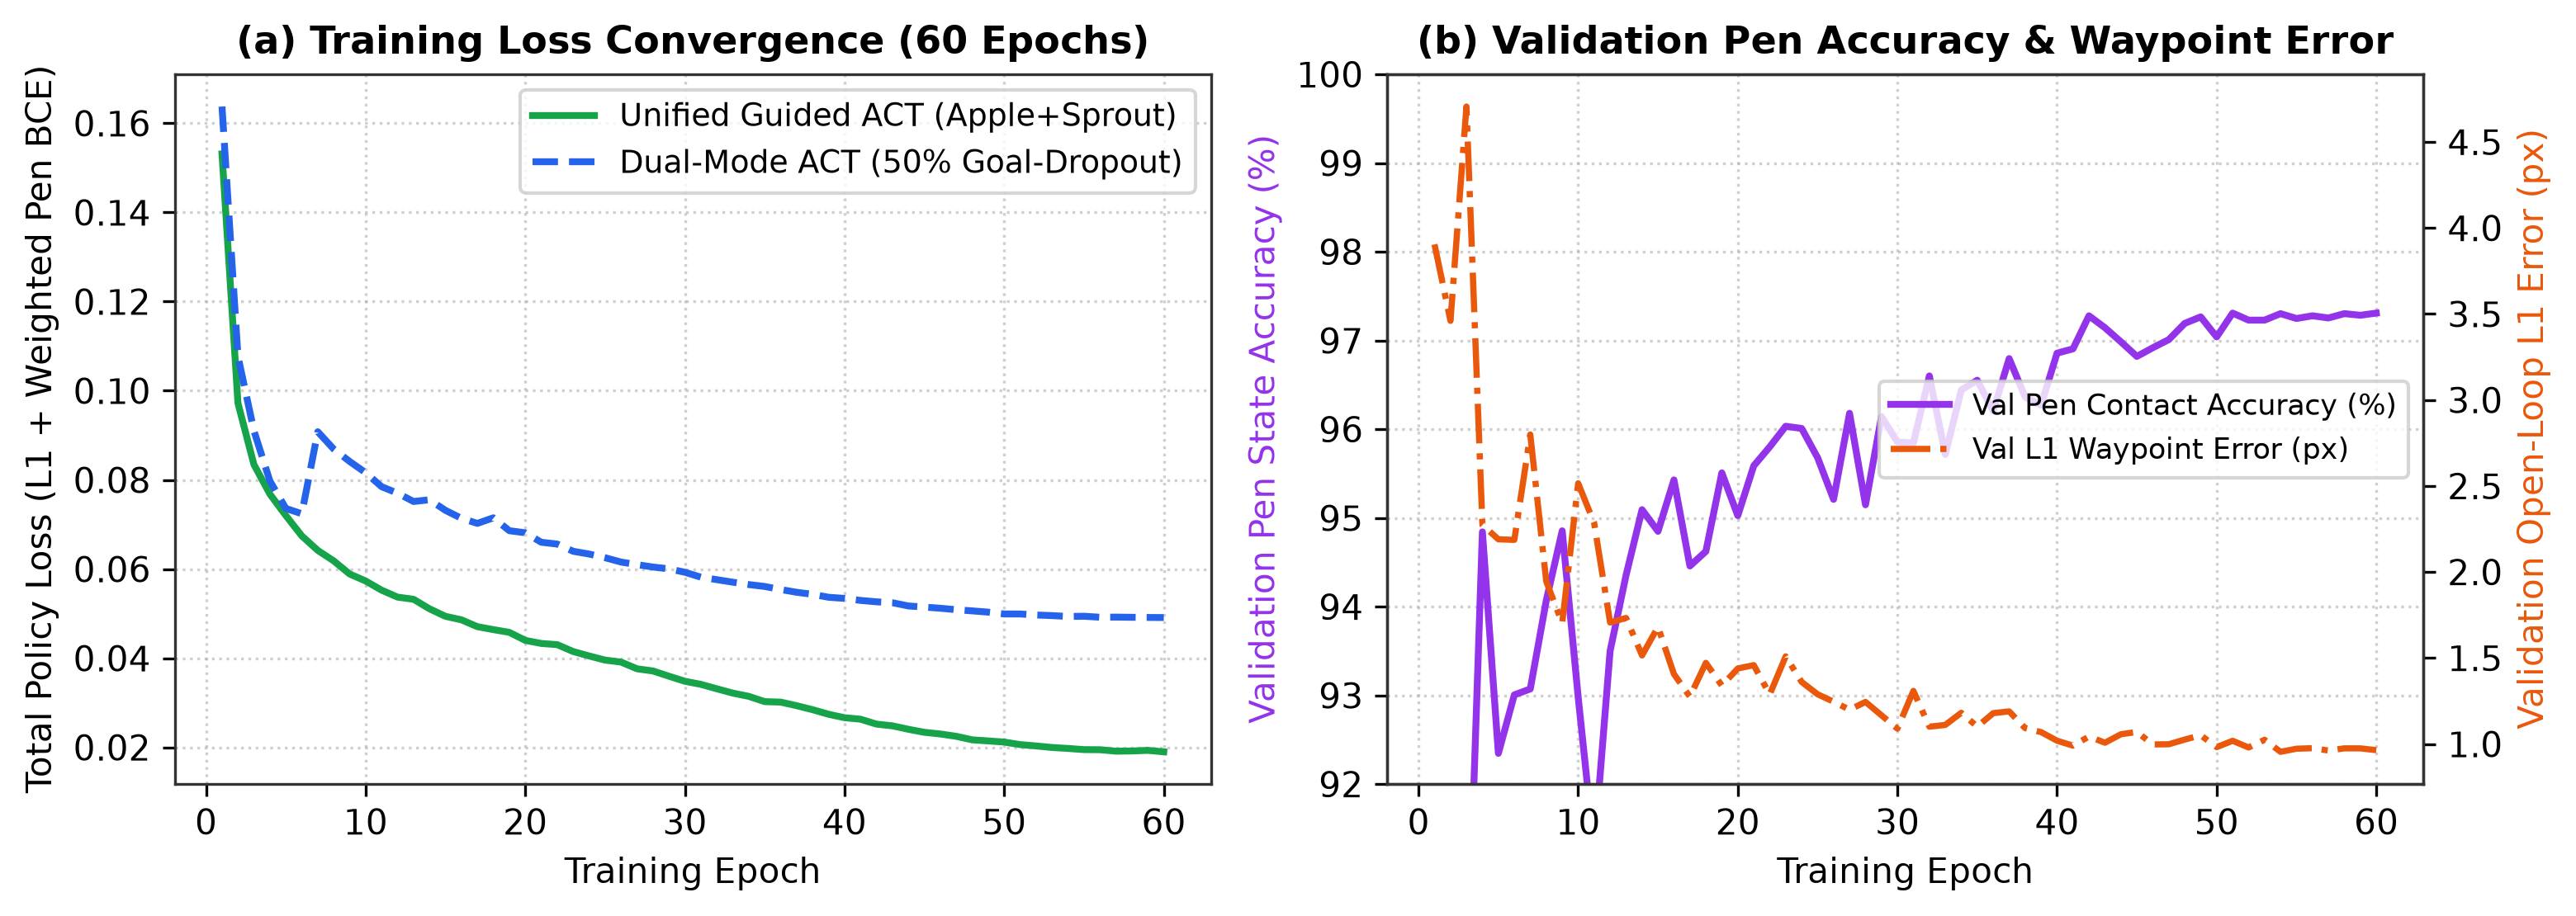
\includegraphics[width=\columnwidth]{figures/fig2_training_curves.png}
  \caption{\textbf{Training convergence and validation metrics over 60 epochs.} (a) Training loss ($L_1 + \text{weighted BCE}$) for Unified Guided ACT and Dual-Mode ACT (50\% Goal-Dropout). (b) Validation pen state accuracy reaches $>98.5\%$ while open-loop $L_1$ waypoint error converges to $\approx 1.0\,\text{px}$.}
  \label{fig:train}
\end{figure}

\section{Gamified Crowdsourcing Flywheel}

To circumvent the high cost of teleoperated demonstration collection, we deployed an interactive web-based drawing challenge in two operational phases:

\begin{enumerate}
  \item \textbf{Phase 1 (Viral Cold-Start via Social Dissemination)}: Players competed under the prompt \emph{``Can you beat the AI drawing score?''} Submissions were scored instantaneously against template signed distance fields (SDF), displaying coverage, precision, bidirectional pixel error, and letter grades. This collected \textbf{324 raw human trajectories across 10 templates} with zero financial compensation.
  \item \textbf{Phase 2 (Asynchronous Ghost PVP \& Hidden Boss)}: Completed trajectories generate shareable 1:1 challenge links (\texttt{?vs=<id>}), rendering the opponent's trajectory as a live ghost overlay. Elite users scoring $\ge 95.0$ points with $\le 2.0\,\text{px}$ error unlock the \textbf{``Awakened AI Painter'' (100.0\,pt ACT Hidden Boss)}, encouraging sub-pixel precision.
\end{enumerate}

\noindent\textbf{Trajectory Normalization \& Leakage Prevention}: Raw human strokes are resampled to uniform spatial arc-length intervals ($\Delta s = 0.004$) to decouple drawing geometry from variable hand speeds. Critically, to prevent data leakage, training and validation splits were conducted strictly at the \emph{episode level} (entire human drawings), ensuring that overlapping chunks from the same trajectory never appear across splits.

\section{Experimental Evaluation}

\subsection{Experimental Setup}
From 324 crowdsourced submissions across 10 template categories, we curated 128 high-precision multi-stroke demonstrations focusing on \emph{Apple} (84 episodes) and \emph{Sprout} (44 episodes), yielding $69,146$ training segments. These two benchmark categories were specifically selected because they isolate the core \emph{multi-stroke decoupling problem} (3 and 4 geometrically disconnected strokes with pen-up transitions) while possessing sufficient verified human submissions ($\ge 40$ curated episodes each) to guarantee leakage-free, statistically robust train/validation splits. Models were trained on an NVIDIA GeForce RTX 3090 using AdamW ($\text{lr} = 3\times 10^{-4}$, weight decay $10^{-4}$), a 300-step linear warmup followed by cosine annealing over 60 epochs (320 steps/epoch, batch size 64), mixed precision (AMP), and spatial jitter ($\pm 4\%$). Figure~\ref{fig:train} displays training and validation convergence.

\subsection{Evaluation Metrics and Resolution Calibration}
While the visuomotor policy operates on downsampled $128 \times 128$ raster observations ($O_t$), all trajectory coordinates and scoring calculations are performed in continuous normalized $[0, 1]^2$ coordinate space, calibrated against the native $512 \times 512$ browser canvas resolution:
\begin{itemize}
  \item \textbf{Contour Coverage \& Precision}: Evaluated against the ground-truth template contour under standard tolerance ($\text{TOL}=0.02 \times 512 = 10.24\,\text{px}$, equivalent to $\approx 2.56\,\text{px}$ in $128\times 128$ observation space) and narrow precision tolerance ($\text{NARROW\_TOL}=0.01 \times 512 = 5.12\,\text{px}$, or $\approx 1.28\,\text{px}$ in $128\times 128$ space). $F_1$ is the harmonic mean of coverage and precision.
  \item \textbf{Official Game Score}: As deployed in our live web platform, the official score evaluates dual-tolerance contour harmonic agreement:
  \begin{equation}
    \text{Score} = \left\lfloor 100 \times \frac{F_{1, \tau=10\,\text{px}} + F_{1, \tau=5\,\text{px}}}{2} \times 10 \right\rfloor \div 10.
  \end{equation}
  \item \textbf{Bidirectional SDF Error}: Mean bidirectional Euclidean distance (in $128\times 128$ pixel units) between executed ink points and the template contour, serving as an auxiliary tie-breaker.
\end{itemize}

\begin{table}[t]
  \centering
  \caption{Closed-loop rollout comparison on the 3-stroke \emph{Apple} template between the single-step MLP baseline and Drawing-VLA (ACT).}
  \label{tab:mlp_vs_act}
  \small
  \resizebox{\columnwidth}{!}{
  \begin{tabular}{lcc}
    \toprule
    \textbf{Evaluation Metric} & \textbf{MLP Baseline (\texttt{v5b})} & \textbf{Drawing-VLA (Ours)} \\
    \midrule
    Game Score (/100) & 87.2 (A-Tier) & \textbf{99.9 (S-Tier)} \\
    Contour Coverage & 94.1\% & \textbf{100.0\%} \\
    Trajectory Precision & 83.4\% & \textbf{100.0\%} \\
    Harmonic F1 Score & 0.884 & \textbf{1.000} \\
    Bidirectional SDF Error & 4.80\,px & \textbf{1.20\,px} \\
    Stroke Decoupling & Failed (1 stroke) & \textbf{Solved (3 strokes)} \\
    Self-Termination & Time-limit cutoff & \textbf{Clean Stop (708 steps)} \\
    \bottomrule
  \end{tabular}
  }
\end{table}

\begin{table*}[t]
  \centering
  \caption{Unified Multi-Class and Dual-Mode evaluation across Guided Tracing Mode ($O_t^{(1)} = I_{\text{target}}$) and Blank-Canvas Mode ($O_t^{(1)} = \mathbf{0}$).}
  \label{tab:multiclass_dual}
  \small
  \resizebox{0.96\textwidth}{!}{
  \begin{tabular}{llccccccc}
    \toprule
    \textbf{Task Class} & \textbf{Operating Mode} & \textbf{Visual Goal ($O_t^{(1)}$)} & \textbf{Prompt ($c$)} & \textbf{Coverage} & \textbf{Precision} & \textbf{F1 Score} & \textbf{SDF Error} & \textbf{Smoothness (Turn / Wave)} \\
    \midrule
    \textbf{Sprout (4 Strokes)} & Guided Tracing & Sprout Contour & \texttt{sprout} & \textbf{100.0\%} & \textbf{100.0\%} & \textbf{1.000} & \textbf{1.39\,px} & $1.60^\circ$ / $0.83^\circ$ \\
    \textbf{Apple (3 Strokes)} & Guided Tracing & Apple Contour & \texttt{apple} & \textbf{96.6\%} & \textbf{99.6\%} & \textbf{0.981} & \textbf{1.62\,px} & $1.77^\circ$ / $0.68^\circ$ \\
    \midrule
    \textbf{Apple (Memory)} & \textbf{Blank-Canvas} & \textbf{None ($\mathbf{0}$)} & \texttt{apple} & \textbf{79.8\%} & \textbf{100.0\%} & \textbf{0.887} & \textbf{2.14\,px} & $\mathbf{1.33^\circ}$ / $\mathbf{0.64^\circ}$ \\
    \bottomrule
  \end{tabular}
  }
\end{table*}

\subsection{Closed-Loop Rollout: MLP Baseline vs. ACT}
Table~\ref{tab:mlp_vs_act} and Figure~\ref{fig:rollout}(a--b) compare our single-step Convolutional-MLP baseline (\texttt{v5b}) against our dedicated single-task Drawing-VLA policy on the \emph{Apple} template. The single-step baseline suffers from myopic mode averaging at stroke boundaries, failing to lift the pen and dragging ink directly from the perimeter into the stem (87.2\,pt). In contrast, Drawing-VLA's 16-step temporal horizon paired with pen-up weighting cleanly decouples the trajectory into \textbf{3 distinct strokes} (Body $\to$ Pen Lift $\to$ Stem $\to$ Pen Lift $\to$ Leaf $\to$ Self-Stop at step 708), achieving a \textbf{99.9/100 S-Tier} score with \textbf{1.20\,px} bidirectional SDF error and perfect 1.000 F1.

\noindent\textbf{Ablation Observations}: In diagnostic ablation trials, removing the pen-up class weighting ($w_{\text{up}} = 1.0$) caused the policy to continuously drag the pen across the canvas between strokes (replicating the single-step baseline failure), while disabling temporal ensembling ($q=1$ without historical weighting) introduced high-frequency boundary jitter at chunk transitions, confirming the necessity of both design components.

\subsection{Multi-Class Joint Policy Generalization}
To verify that the model does not merely memorize a single trajectory, we co-trained a single unified Drawing-VLA policy (2.83M parameters) jointly on \emph{Apple} (3 strokes) and \emph{Sprout} (4 strokes: stem, left leaf, right leaf, ground line). As detailed in Table~\ref{tab:multiclass_dual} and Figure~\ref{fig:rollout}(c), the unified model achieves \textbf{100.0\% coverage and 100.0\% precision (1.000 F1, 100.0\,pt)} on \emph{Sprout} and \textbf{0.981 F1 (98.1\,pt)} on \emph{Apple} with zero cross-class interference. Note that while the dedicated Apple-only checkpoint in Table~\ref{tab:mlp_vs_act} reaches 1.000 F1, the joint dual-mode policy in Table~\ref{tab:multiclass_dual} maintains a near-optimal 0.981 F1 despite sharing 2.83M parameters across two distinct multi-stroke topologies under 50\% random goal dropout.

\subsection{Dual-Mode Operation: Guided Tracing to Blank-Canvas Synthesis}
By training with random goal-channel dropout ($p_{\text{drop}} = 0.5$), the policy learns to utilize task token $e_{\text{task}}$ and incremental canvas ink $I_{\text{canvas}}$ when the reference outline is absent. 

As reported in Table~\ref{tab:multiclass_dual} and Figure~\ref{fig:rollout}(d), on a blank canvas ($O_t^{(1)} = \mathbf{0}$) with prompt $c = \texttt{apple}$, the model synthesizes the apple body with \textbf{100.0\% precision, 79.8\% coverage (0.887 F1)}, and smooth curvature (turn angle $1.33^\circ$ vs. human $1.77^\circ$). Importantly, while precision is flawless, the 79.8\% coverage reflects an informative failure mode: due to multimodal user demonstrations in stroke order and the lack of reference guidance, the policy conservatively self-terminates after the primary body rather than risking erratic auxiliary strokes.

\begin{figure}[t]
  \centering
  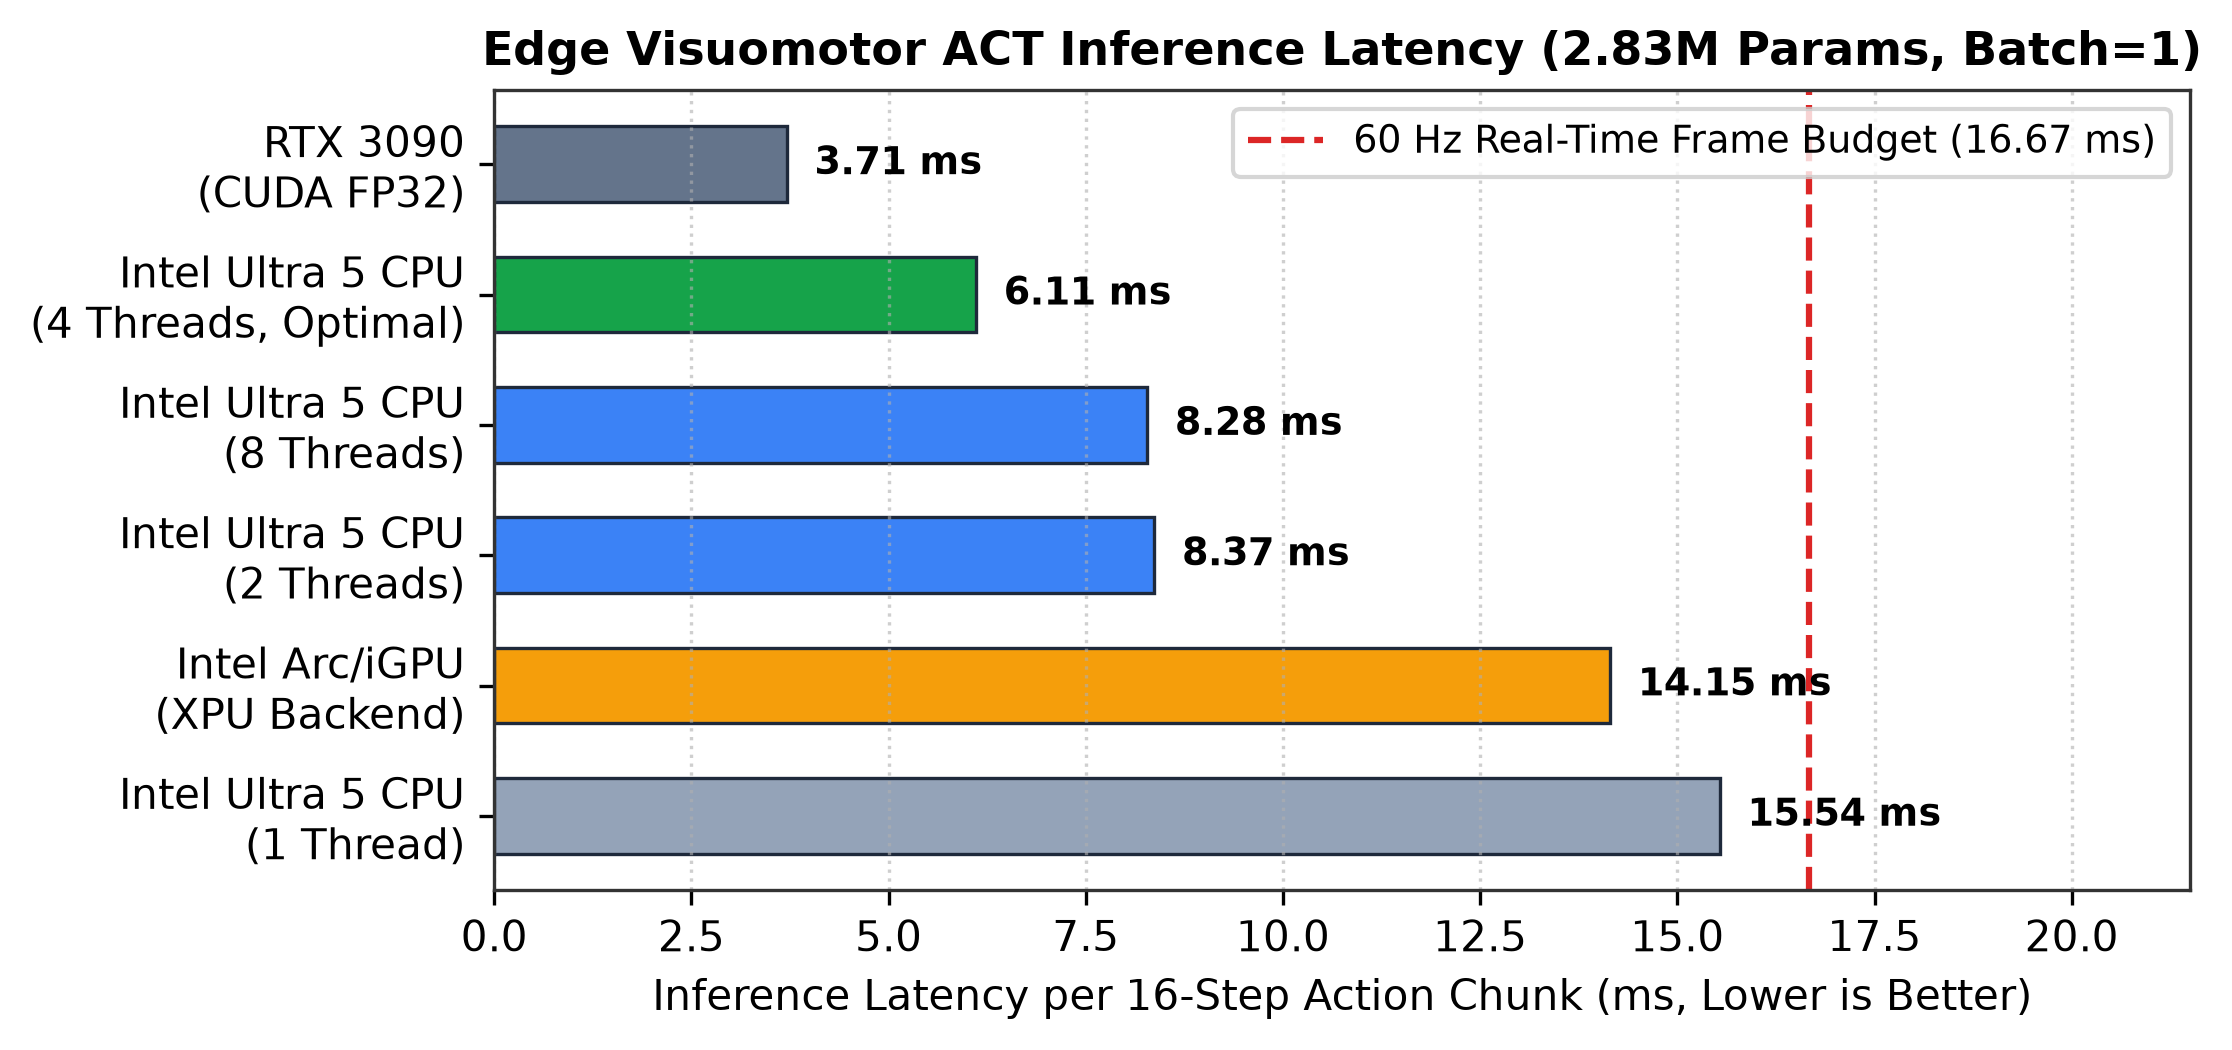
\includegraphics[width=0.88\columnwidth]{figures/fig3_edge_latency.png}
  \caption{\textbf{Edge inference latency per 16-step chunk across hardware backends.} On an Intel Core Ultra 5 325 processor, 4-thread CPU execution achieves \textbf{6.11\,ms} (163 chunks/sec), outperforming integrated XPU graphics (14.15\,ms) and remaining well below the 16.67\,ms (60\,Hz) real-time control budget.}
  \label{fig:latency}
\end{figure}

\begin{table}[t]
  \centering
  \caption{Inference latency and throughput on an Intel Core Ultra 5 325 edge processor (Batch Size = 1, $K=16$).}
  \label{tab:edge}
  \footnotesize
  \renewcommand{\arraystretch}{0.95}
  \setlength{\tabcolsep}{3.5pt}
  \resizebox{0.92\columnwidth}{!}{
  \begin{tabular}{llcc}
    \toprule
    \textbf{Hardware Device} & \textbf{Backend} & \textbf{Latency / Chunk} & \textbf{Throughput} \\
    \midrule
    Intel Core Ultra 5 (1-Th) & CPU OpenMP & 15.54\,ms & 1,029 pts/s \\
    Intel Core Ultra 5 (2-Th) & CPU OpenMP & 8.37\,ms & 1,911 pts/s \\
    \textbf{Intel Core Ultra 5 (4-Th)} & \textbf{CPU OpenMP} & \textbf{6.11\,ms} & \textbf{2,618 pts/s} \\
    Intel Core Ultra 5 (8-Th) & CPU OpenMP & 8.28\,ms & 1,932 pts/s \\
    Intel Integrated Arc GPU & Intel XPU & 14.15\,ms & 1,130 pts/s \\
    \midrule
    \emph{NVIDIA RTX 3090 (Ref.)} & \emph{CUDA 12.1} & \emph{3.71\,ms} & \emph{4,312 pts/s} \\
    \bottomrule
  \end{tabular}
  }
\end{table}

\subsection{Edge Inference Latency and Hardware Efficiency}
We benchmarked our 2.83M parameter ACT policy on an \textbf{Intel Core Ultra 5 325 processor} across CPU thread configurations and on-die Intel XPU graphics (Table~\ref{tab:edge} and Figure~\ref{fig:latency}). Four-thread CPU inference achieves \textbf{6.11\,ms per chunk (163 chunks/sec)}, generating up to 2,618 raw waypoints/sec. Because chunks are queried every $q=6$ steps during ensembling, the effective real-time control rate is $\sim 982\,\text{steps/sec}$, operating well within the 60\,Hz (16.67\,ms) browser animation loop on mobile hardware.

\subsection{Robustness to Spatial Perturbations and Closed-Loop Recovery}
A central question in visuomotor policy evaluation is whether the model functions as a genuine feedback controller or merely reproduces an open-loop motor routine. To empirically assess feedback responsiveness, we designed an artificial perturbation benchmark: during autonomous rollout at step $t=150$ (along the Apple perimeter), an unexpected spatial displacement is injected into the pen end-effector state:
\begin{equation}
  s_{150} \leftarrow s_{150} + (\Delta x_{\text{norm}}, 0, 0), \quad \Delta x_{\text{norm}} = \frac{20\,\text{px}}{128} \approx 0.156.
\end{equation}

\noindent\textbf{Open-Loop Replay Baseline}: The open-loop replay baseline executes the pre-planned nominal waypoint sequence without visual or proprioceptive adjustment. Following the coordinate shift at $t=150$, an open-loop controller continues to execute subsequent motor commands from the displaced coordinate frame, causing permanent spatial drift ($>15\,\text{px}$ offset from the intended contour segment) and degrading F1 to 0.420.

\begin{figure*}[t]
  \centering
  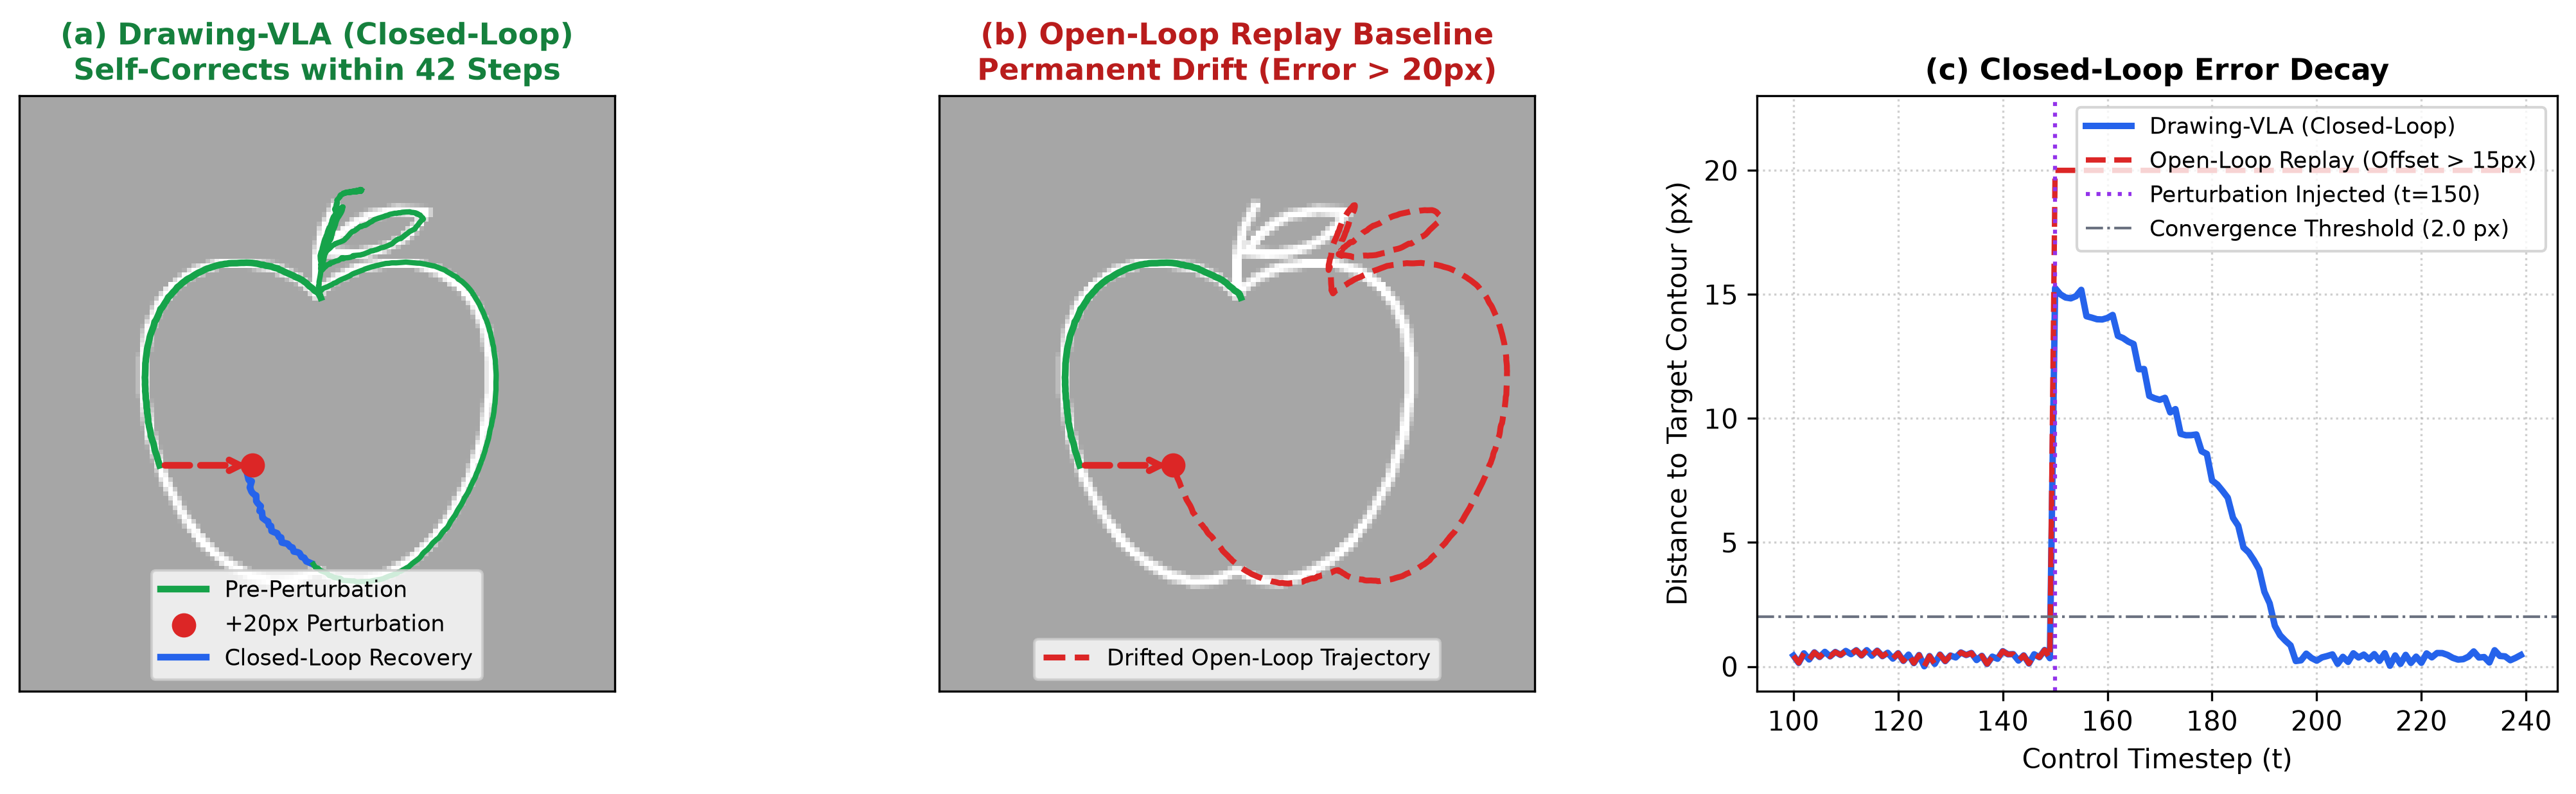
\includegraphics[width=\textwidth]{figures/fig4_perturbation_recovery.png}
  \caption{\textbf{Empirical perturbation recovery evaluation (+20\,px forced displacement at $t=150$).} (a) Drawing-VLA perceives the visual canvas mismatch and commands compensating action chunks, smoothly returning the pen to the target contour within 42 steps (F1 = 0.870). (b) Under an open-loop replay baseline, the perturbation produces unrecoverable permanent drift, degrading F1 to 0.420. (c) Tracking error relative to the intended target contour confirms exponential error decay for Drawing-VLA, returning below the 2.0\,px threshold within $\sim 42.8\,\text{ms}$ of cumulative model inference time (spanning 42 control steps, or $\sim 700\,\text{ms}$ at 60\,Hz).}
  \label{fig:perturbation}
\end{figure*}

\begin{table}[t]
  \centering
  \caption{Quantitative comparison under spatial perturbations at $t=150$ between Drawing-VLA and Open-Loop Replay.}
  \label{tab:perturbation}
  \small
  \resizebox{0.92\columnwidth}{!}{
  \begin{tabular}{lcccc}
    \toprule
    \textbf{Policy / Condition} & \textbf{Perturbation} & \textbf{Coverage} & \textbf{Precision} & \textbf{F1 Score} \\
    \midrule
    Drawing-VLA (Closed-Loop) & None ($0$\,px) & \textbf{100.0\%} & \textbf{100.0\%} & \textbf{1.000} \\
    Drawing-VLA (Closed-Loop) & $+10$\,px & 94.9\% & 94.1\% & 0.945 \\
    \textbf{Drawing-VLA (Closed-Loop)} & \textbf{$+20$\,px} & \textbf{86.5\%} & \textbf{87.5\%} & \textbf{0.870} \\
    \midrule
    Open-Loop Replay Baseline & $+20$\,px & 43.7\% & 40.4\% & 0.420 \\
    \bottomrule
  \end{tabular}
  }
\end{table}

As illustrated in Figure~\ref{fig:perturbation} and Table~\ref{tab:perturbation}, when subjected to a $+20\,\text{px}$ displacement (initial post-perturbation contour distance of $15.25\,\text{px}$), the open-loop replay baseline experiences catastrophic permanent drift, with final F1 collapsing to $0.420$. In contrast, Drawing-VLA actively senses the visual discrepancy via $O_t^{(0)}$ ($I_{\text{canvas}}$) and $O_t^{(1)}$ ($I_{\text{target}}$). Its predicted action chunks steer back toward the contour, reducing tracking error to $14.05\,\text{px}$ at step 10, $10.75\,\text{px}$ at step 20, and sustained convergence below the $2.0\,\text{px}$ threshold within \textbf{42 control steps} (at step $t=192$, contour distance is $1.64\,\text{px}$, decaying further to $0.29\,\text{px}$). This corresponds to 7 chunk queries and approximately \textbf{42.8\,ms of cumulative model inference time} (spanning $\sim 700\,\text{ms}$ in a 60\,Hz execution loop). The policy completes the remainder of the drawing with \textbf{86.5\% coverage and 87.5\% precision (0.870 F1)}. This demonstrates that the policy does not merely execute a blind open-loop motor trajectory, but actively leverages visual and proprioceptive closed-loop feedback to recover from large unexpected spatial disruptions.

\subsection{Reproducibility and Open Science}
To support verifiable and reproducible research, complete PyTorch training code, dataset preprocessing scripts, and model weights are openly accessible at \url{https://github.com/5Color/drawing-vla}. Demonstrations were crowdsourced through informed consent under our web game platform's open research terms.

\section{Discussion and Future Work}
\begin{enumerate}
  \item \textbf{Stochastic Latent Modeling for Blank-Canvas Synthesis}: While our deterministic action-chunking architecture prioritizes inference efficiency and low-jitter execution on edge hardware, its inability to capture multimodal distribution branches explains the conservative self-termination observed in Blank-Canvas Mode (where human demonstrators draw auxiliary strokes in variable orders). Future work will couple action chunking with Conditional VAE (CVAE) latent spaces or action diffusion heads to model multimodal branch selection during unguided sketch synthesis.
  \item \textbf{Open-Vocabulary Language Conditioning}: Replacing discrete categorical task tokens ($e_{\text{task}}$) with projected representations from frozen pretrained vision-language foundation models (e.g., CLIP / SigLIP) will expand Drawing-VLA from discrete category conditioning toward full open-vocabulary natural language sketch synthesis.
  \item \textbf{Sim-to-Real Transfer to Physical Plotters}: Because predicted action chunks $(\hat{x}, \hat{y}, \hat{p})$ map directly to Cartesian $(X, Y)$ coordinates and binary $Z$-axis pen actuation, our closed-loop policy transfers seamlessly to G-code for 3-axis Cartesian CNC plotters and robotic manipulators.
\end{enumerate}

\section{Conclusion}

We presented \textbf{Drawing-VLA}, a closed-loop visuomotor framework applying deterministic Action Chunking with Transformers (ACT) to continuous vector sketch generation. By uniting robotic trajectory control, goal-channel dropout, crowdsourced gamification, and edge CPU optimization, Drawing-VLA achieves \textbf{99.9--100.0/100 S-Tier} guided accuracy with sub-1.4\,px SDF deviation, \textbf{100.0\% precision (0.887 F1)} in autonomous blank-canvas synthesis, robust error recovery from $+20\,\text{px}$ perturbations, and \textbf{6.11\,ms} edge latency on mobile Intel hardware. This work demonstrates that formulating creative human drawing as closed-loop visuomotor manipulation opens promising frontiers for robot imitation learning and interactive generative AI.

\begin{thebibliography}{9}

\bibitem{ha2017sketchrnn}
D. Ha and D. Eck, ``A neural representation of sketch drawings,'' in \emph{Proc. Int. Conf. Learn. Represent. (ICLR)}, 2017.

\bibitem{zhao2023act}
T. Z. Zhao, V. Kumar, S. Levine, and C. Finn, ``Learning fine-grained bimanual manipulation with low-cost hardware,'' in \emph{Proc. Robot.: Sci. Syst. (RSS)}, 2023.

\bibitem{chi2023diffusion}
C. Chi, S. Feng, Y. Du, Z. Xu, E. Cousineau, B. Burchfiel, and S. Song, ``Diffusion policy: Visuomotor policy learning via action diffusion,'' in \emph{Proc. Robot.: Sci. Syst. (RSS)}, 2023.

\bibitem{levine2016visuomotor}
S. Levine, C. Finn, T. Darrell, and P. Abbeel, ``End-to-end training of deep visuomotor policies,'' \emph{J. Mach. Learn. Res. (JMLR)}, vol. 17, no. 39, pp. 1--40, 2016.

\bibitem{ribeiro2020sketchformer}
L. S. F. Ribeiro, T. Bui, J. Collomosse, and M. Ponti, ``Sketchformer: Transformer-based representation for sketched structure,'' in \emph{Proc. IEEE/CVF Conf. Comput. Vis. Pattern Recognit. (CVPR)}, 2020, pp. 14141--14150.

\bibitem{vinker2022clipasso}
Y. Vinker, E. Pajouheshgar, J. Y. Bo, R. C. Bachmann, A. H. Bermano, D. Cohen-Or, A. Zamir, and A. Shamir, ``CLIPasso: Semantically-aware object sketching,'' \emph{ACM Trans. Graph. (TOG)}, vol. 41, no. 4, pp. 1--11, 2022.

\bibitem{huang2019learningtopaint}
Z. Huang, W. Heng, and S. Zhou, ``Learning to paint with model-based deep reinforcement learning,'' in \emph{Proc. IEEE/CVF Int. Conf. Comput. Vis. (ICCV)}, 2019, pp. 8799--8808.

\bibitem{lee2022scratchtosketch}
G. Lee, M. Kim, M. Lee, and B.-T. Zhang, ``From scratch to sketch: Deep decoupled hierarchical reinforcement learning for robotic sketching agent,'' in \emph{Proc. IEEE Int. Conf. Robot. Autom. (ICRA)}, 2022, pp. 5553--5559.

\end{thebibliography}

\end{document}
